%%%%%%%%%%%%%%%%%%%%%%%%%%%%%%%%%%%%%%%%%%%%%%%%%%%
%% Modèle de rapport pédagogique, doublé d'un tutoriel LaTeX
%% Vincent Labatut 2014-22 <vincent.labatut@univ-avignon.fr>
%%%%%%%%%%%%%%%%%%%%%%%%%%%%%%%%%%%%%%%%%%%%%%%%%%%
%% Classe du document

\documentclass{ceri/sty/rapport}
% \documentclass[handout]{ceri/sty/rapport}
% \documentclass[light]{ceri/sty/rapport}
% \documentclass[full]{ceri/sty/rapport}
% \documentclass[blue]{ceri/sty/rapport}

\setcounter{section}{0}
\usepackage{graphicx}
\graphicspath{{images}}
\usepackage{booktabs}

%%%%%%%%%%%%%%%%%%%%%%%%%%%%%%%%%%%%%%%%%%%%%%%%%%%
%% Informations générales
%%%%%%%%%%%%%%%%%%%%%%%%%%%%%%%%%%%%%%%%%%%%%%%%%%%
%TODO Formation concernée : à compléter.
% Exemples : Licence d'Informatique, Master d'Informatique.
\major{CentraleSupélec}

%TODO Parcours ou spécialité de la formation
% Exemples pour la licence : Systèmes et Réseaux Informatiques, Ingénierie Logicielle.
% Exemples pour le master : Ingénierie du Logiciel pour la Société Numérique, Réseaux Informatiques et Services Mobiles.
\specialization{FISA}

%TODO UE concernée par le rapport (à modifier).
% exemple : Projet Algorithmique
\course{SIP}

%TODO UCE concernée par le rapport (à modifier, optionnel).
%\subcourse{RedActed}

%TODO Titre du document, à adapter.
\title{Rapport de TP}
\subtitle{Développement d'une API pour la DGSE} % seulement si nécessaire

%TODO Liste des auteurs
\author{
Ewen DENIAU\\
Nathan LEROUGE
}

%TODO Liste des encadrants, responsables d'UE, etc. (optionnel)
%\advisor[Responsables]{ % indiquez ici le rôle (par défaut : "Encadrement")
%	Prénom5 Nom5 \\ % il faut aller à la ligne entre chaque encadrant, comme pour les auteurs
%	Prénom6 Nom6 \\
%	Prénom7 Nom7
%}
\advisor[Professeur]{ % indiquez ici le rôle (par défaut : "Encadrement")
 Sébastien KILIAN\\
 Fanny DIJOUD\\
 Erwan FASQUEL\\
 Lucas GIORDANI
}
%TODO Groupe des auteurs
% Optionnel : seulement si le travail est réalisé en groupe (en l'absence de groupe, ne définissez pas la macro)
% Exemple : Groupe 1, G12, etc.
%\group{Nom/numéro du groupe de travail}

% Date de finalisation du rapport. 
% La valeur par défaut, qui est recommandée, est la date du jour.
%\date{\today}
%\dateUpdt{}

% affiliations des auteurs (pour un rapport de recherche uniquement)
% \affiliations{
%     \textsuperscript{1} Laboratoire Informatique d'Avignon -- LIA EA 4128 \\
%     \textsuperscript{2} Laboratoire Biens, Normes, et Contrats - LBNC EA 3788
% }

% Il est possible de définir un résumé du document (optionnel) avec la commande \resume comme ci-dessous. 
% Si la commande n’apparaît pas, le résumé n'est pas inséré dans le document.
% \summary{Ce document est une introduction à \LaTeX{}. Il s'agit à la fois d'un tutoriel décrivant les principales fonctionnalités de ce système de composition de documents, et d'un modèle servant d'exemple à l'élaboration d'un document. Il utilise le fichier de mise en forme fourni pour l'écriture de rapports dans le cadre des enseignements donnés au CERI, Université d'Avignon.}
% \summary{Ce document est la première version du rapport à produire dans le cadre du stage de fin d'année en Licence 3 MIS - CMI. Il va introduire ce qui a pu être réalisé lors du premier mois du stage.}



%%%%%%%%%%%%%%%%%%%%%%%%%%%%%%%%%%%%%%%%%%%%%%%%%%%
%% Bibliographie
%%%%%%%%%%%%%%%%%%%%%%%%%%%%%%%%%%%%%%%%%%%%%%%%%%%
% Désigne le fichier bibliographique à utiliser
% \addbibresource{bibliographie.bib}



%%%%%%%%%%%%%%%%%%%%%%%%%%%%%%%%%%%%%%%%%%%%%%%%%%%
%% Début du document
%%%%%%%%%%%%%%%%%%%%%%%%%%%%%%%%%%%%%%%%%%%%%%%%%%%
\begin{document} 

% Création de la page de titre.
\maketitle

% Justification moins stricte : empêche certains mots de dépasser dans la marge
\sloppy      

\section{Introduction}
Ce document est le rapport de rendu du TP de SIP.
TP dans lequel nous devions développer une API où nous collections et assemblons plusieurs informations concernant des vols et des aéroports.

Le travail a été effectué par Ewen Deniau et Nathan Lerouge dans le cadre du cours de SIP.
Les scripts ont été programmés en Python, avec les librairies suivantes :
\begin{itemize}
    \item Pandas
    \item SQLite
    \item Flask
\end{itemize}

Vous pourrez retrouver le code sur le repo suivant : \href{https://github.com/Bismuth10K/flights-api}{Bismuth10K/flights-api}

\section{Database design}
\subsection{Question 1}
La première tâche de ce projet consiste à élaborer un diagramme entité-relation (ER) pour identifier les différentes entités et les relations qui existent entre elles. Ce diagramme nous permet de visualiser les interactions entre des éléments essentiels comme les compagnies aériennes, les vols, les aéroports, les utilisateurs et les pays. Par exemple, un vol est caractérisé par un aéroport de départ, une heure de départ, un aéroport et une heure d'arrivée, le type d'avion utilisé pour ce vol et son prix. Une fois ce modèle ER conçu, nous le traduisons en un modèle relationnel sous forme de tables dans une base de données relationnelle.

Chaque table doit contenir une clé primaire pour garantir l'unicité des enregistrements (par exemple, \texttt{flight\_id} pour les vols).
Les clés étrangères assurent la cohérence des relations entre les tables (comme un champ \texttt{isao\_country\_code} dans une table d'aéroports pour lier chaque aéroport au pays dans lequel il est situé).
Nous adoptons la troisième forme normale (3NF), une norme de structuration qui permet d'éviter les redondances et de minimiser les anomalies lors des insertions, suppressions ou mises à jour.

\begin{figure}[h]
    \centering
    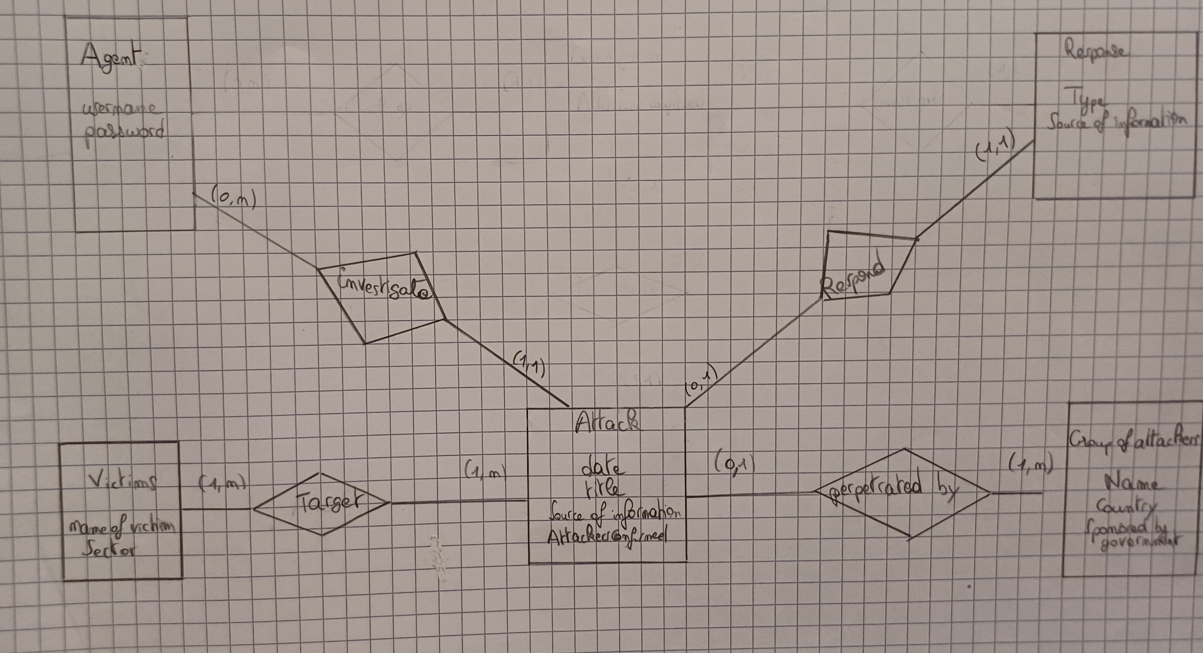
\includegraphics[width=0.85\linewidth]{images/diag_er.png}
    \caption{Diagramme entité-relation}
    \label{fig:diag_er}
\end{figure}

\begin{figure}[h]
    \centering
    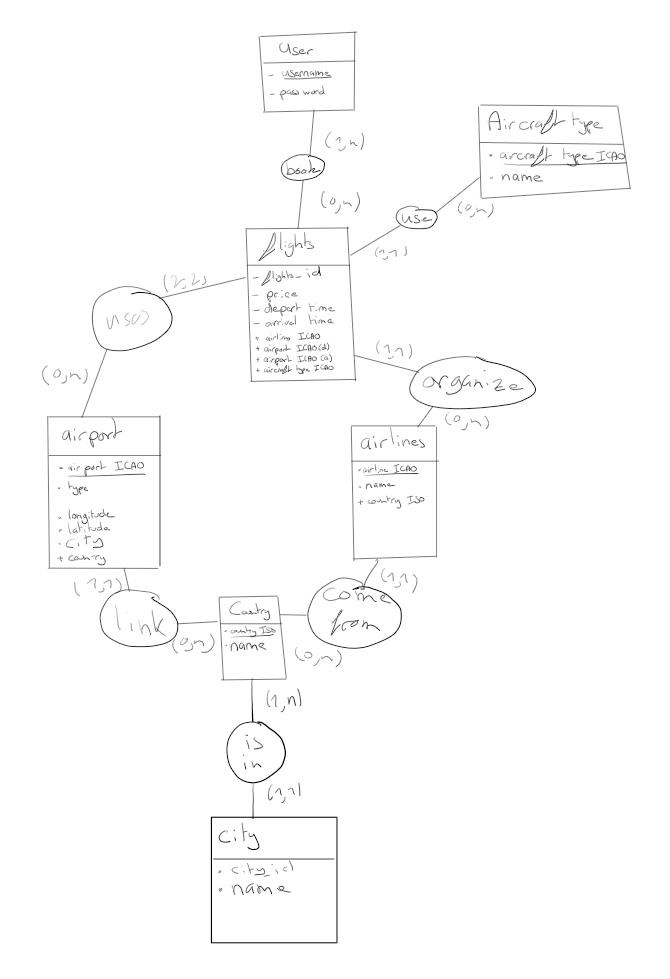
\includegraphics[width=0.85\linewidth]{images/diag_phys.png}
    \caption{Modèle physique}
    \label{fig:diag_phys}
\end{figure}

\section{\textit{Create the database}}
\subsection{Question 2 et 3}
Ce script permet de séparer le fichier all.csv en différentes tables sous la forme d'un \textit{dataframe} pandas afin de structurer les données.
Ainsi ce script renvoie une liste de \textit{dataframes} pandas représentant chacun une table, calquant le diagramme ER. 

\subsection{Question 5}
Ce script permet de créer la base de données qui sera utilisée plus tard. 
L'organisation de celle-ci se base toujours sur le Diagramme ER en y rajoutant des tables si nécessaire (\textit{e.g.} la table \texttt{Booking} liant \texttt{User} et \texttt{Flights}).

\subsection{Question 6}
À l'aide des \textit{dataframes} pandas et des tables SQL vides dans notre database, nous remplissons les tables avec les informations des \textit{dataframes}.
Pour cela, nous utilisons la commande SQL : \texttt{INSERT INTO ... VALUES ...}.

Pour certaines tables, une clé primaire "…\_id" était nécessaire pour distinguer tous les vols, tous les utilisateurs ou toutes les réservations.
Pour garantir l'unicité des identifiants, nous avons utilisé un incrémenteur automatique, ici le numéro de ligne.

\subsection{Question 7}
Dans la fonction \texttt{init\_database()}, nous devons maintenant appeler correctement la fonction \texttt{populate\_database()}.
Cette fonction a besoin de \texttt{cursor} afin d'exécuter des requêtes SQL, et de \texttt{conn} qui permet la connexion à la BDD, ainsi que la liste des \textit{dataframes} pandas contenant toutes les informations à remplir dans les tables SQL.

\section{\textit{First communications with the database}}
\subsection{Question 8}
Nous avons lu, ce fut très fructueux.

\subsection{Question 9}
Il manquait l'appel de la méthode \texttt{conn.commit()}.
Le \textit{commit} sert à confirmer les modifications effectuées sur la base de données.

\subsection{Question 10}
Nous sommes dans le regret de vous annoncer qu'aucune erreur nous a marqué à l'heure où nous écrivons ces lignes.
Nous écrivons le rapport après avoir fini le code, et nous nous sommes organisés de façon à ce que nous ignorions complètement ce qui était demandé dans cette question.

En vous remerciant de votre compréhension.

\subsection{Question 11}
Nous vous laissons lire l'implémentation.
Nous avons aussi pris le soin de hasher le mot de passe comme demandé plus tard.

\subsection{Question 12}
Quand nous essayons de modifier le mot de passe d'un utilisateur inexistant, cela ne marche pas.
L'utilisateur n'est pas trouvé dans la BDD.



\section{\textit{Database manipulation}}
\subsection{Question 13}
Cette série de fonction permet d'utiliser au mieux la database pour des demandes récurrentes.
Par exemple : connaître le nom d'une ville lorsqu'on ne connaît que son code ISO, connaître toutes les informations d'un aéroport simplement avec son id.
Cela permet d'utiliser la database efficacement.

\section{\textit{Create the first API routes}}
\subsection{Question 14}
Ce script créé l'application (i.e. le serveur web) sur le port 5000 du serveur où sera hébergé le code. Le serveur web est géré par la librairie Flask.

\subsection{Question 15}
Pour obtenir tous les \texttt{users}, il faut juste aller à la racine du blueprint \texttt{users} comme en témoigne la ligne suivante :

\begin{lstlisting}[language=python]
@users_bp.route("/", methods=["GET"])
def get_all_users():
    <code>
\end{lstlisting}

Le premier paramètre de la méthode route définit la suite de l'url, en l'occurence un slash simple donc la racine. Nous devons donc accéder à l'url suivant : \texttt{\url{http://localhost:5000/users/}}

Et enfin, il s'agit d'une requête \texttt{GET}.

\subsection{Question 16}
Pour les questions de ce genre, nous vous redirigeons vers le script \texttt{test\_requests.py} et d'appeler les fonctions de votre choix.

\subsection{Question 17}
Nous vous redirigeons vers le script correspondant pour voir l'implémentation.

\section{\textit{Help to debug}}
\subsection{Question 18}
Nous vous redirigeons vers le script correspondant pour voir l'implémentation.
Nous avons aussi implémenté des fonctions supplémentaires afin de nous simplifier le travail et de compléter des fonctions non réalisés dans la bibliothèque db.

\section{\textit{Remaining routes}}
\subsection{Question 19}
Même réponse que pour la 18, et nous y avons aussi créés des fonctions supplémentaires.

Idéalement, toutes ces fonctions devraient être confirmées par des tests unitaires.
N'étant pas le sujet principal de ce TP, nous continuons ainsi.

\section{\textit{Securing the API}}
\subsection{Question 20 - 21}
Nous vous laissons aussi voir l'implémentation. 
Elle n'est pas très poussée et suis globalement la documentation de la librairie.

Ensuite, nous appelons les fonctions adaptées dans la fonction \texttt{insert\_user()}.

\subsection{Question 22 - 24}
Les tokens sont implémentés et fonctionnent correctement.
Nous vous laissons voir l'implémentation encore une fois.

Pour le décorateur, nous avons surtout décidé de le mettre sur des fonctions ayant besoin d'une forme d'authentification.
Par exemple, nous ne pouvons pas laisser n'importe qui observer la liste des voyageurs d'un vol, car la protection des données n'est pas respectée.
Nous sommes aussi partis du principe que les agents allaient aussi avoir des \textit{tokens}.

Certaines fonctions n'ayant pour but que de chercher tous les vols (par exemple) n'ont pas besoin de \textit{tokens}.
Puisqu'ils permettent à une personne d'observer les vols avant d'acheter, et donc de ce faire un compte.

Nous souhaitons vous faire remarquer deux choses :

\begin{itemize}
    \item Premièrement, il serait pertinent de modifier les fonctions afin de lire l'utilisateur dans le \textit{token}. 
    Ainsi, nous pouvons lui assigner directement une réservation à son nom.
    \item Secondement, nous avons mentionné les agents.
    Nous pensons que rajouter des droits et des privilèges en fonction des gens rajouteraient une couche de sécurité. 
\end{itemize}


\begin{beware}[Remarque]
Lors de l'implémentation du \textit{token}, nous avons remarqué que le code fourni appliquait un \texttt{split} et prenait le second élément pour récupérer le \textit{token}.
Après concertation avec madame Dijoud, j'ai eu son accord pour modifier cette partie afin de récupérer directement le \textit{token} sans opérations supplémentaires.
\end{beware}

%%%%%%%%%%%%%%%%%%%%%%%%%%%%%%%%%%%%%%%%%%%%%%%%%%%
%% Crédits
%%%%%%%%%%%%%%%%%%%%%%%%%%%%%%%%%%%%%%%%%%%%%%%%%%%
\section{Crédits}
Nous voulons remercier les professeurs de leurs aides et de leurs cours lors du développement de ce TP.
Nous remercions aussi tous les forums et tutos qui existent en ligne et qui nous ont aidé.

\subsection{Document}
Le template du document provient de Vincent Labatut (\url{vincent.labatut@univ-avignon.fr}) tel que modifié par Simon Leclercq (\url{leclercq.e2102543@etud.univ-ubs.fr}).
Les modifications supplémentaires ainsi que la page de garde proviennent d'Ewen Deniau (\url{ewen.deniau@student-cs.fr}).

%%%%%%%%%%%%%%%%%%%%%%%%%%%%%%%%%%%%%%%%%%%%%%%%%%%
%% Bibliographie
%%%%%%%%%%%%%%%%%%%%%%%%%%%%%%%%%%%%%%%%%%%%%%%%%%%
\nocite{*}
% \MyBibliography

\end{document}
